\cleardoublepage
\counterwithout{figure}{section}
\counterwithout{table}{section} 
\counterwithout{equation}{section}
\counterwithin{figure}{chapter}
\counterwithin{table}{chapter} 
\counterwithin{equation}{chapter}


\chapter{Introduction}
\label{sec:problemstellung}
 Only in Germany more than 1 Million teeth are replaced annually. The replacement procedure is accomplished with an implantation of the tooth replica to provide the aesthetics and the function of the natural tooth. Ancient Egyptians used tooth shaped ivory to regain the function of the missing teeth. Today the technology has evolved to a point where the dental replacement for a single tooth is an assembly of three parts, which  are to be seen in Figure 1.1. The implant is the part which is screwed to the lower jaw bone (mandible) and anchors the whole replacement assembly to the chin. The preferred material used for the implant are titanium in the EU and tantalum in the US. The enhanced osseointegration of the porous implant material surface, biocompatibility of the ceramic interface, formed due to the surface oxidation a Young's Modulus, which is similar to the human bone are the main reasons for titanium and tantalum to be the prime materials for this purpose. The abutment takes on the task of a fitting  for the crown and is made of the same material as the implant.
  \begin{figure}[h]
 	\centering
 	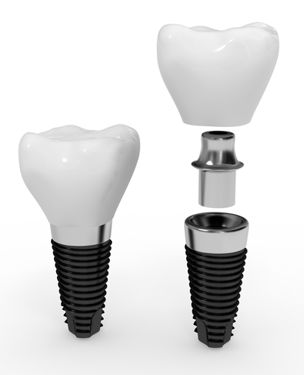
\includegraphics[width=0.4\textwidth]{grafiken/implant.png}
 	\caption{Single tooth replacement}
 	\label{fig:bild1}
 \end{figure} 
 
 The crown of the tooth replacement is the part which imitates the visual qualities of the tooth. There are several material, which a crown can be made of or assembled from. The most popular crown material dominating the market is the Yttria-stabilized zirconia (YSZ), which has a cubic fluorite crystal structure and is going to be referred as zirconia in the frame of this work. However, but Zirconia in its pure form is plain white so coloring the crown is necessary.Dentist are using such a shade guide for a side-by-side comparison to determine the color and the shade of the teeth.One can observe that there are 4 color groups A B C and D and each of these colors have 4 shades coded with the numbers from 1 to 4. Where 1 is the least and 4 is the most saturated shade for each color. 
 


\chapter{State of the Research}
\label{sec:stand_forschung}

\section{Drop Deployment}


\subsection{Piezoelectric}


\subsection{Electromagnetic}
\label{sec:freiheitsgrad_eines_getriebes}




\section{Coloring behavior of the ceramic}
\label{sec:grundlagen_für_die_kinematischen_betrachtungen}


\chapter{State of the Technology}
\label{sec:stand_technik}
On the left side you can see a cutout of a lab card. Dentists mark different areas of the crown with different colors from the guide for the technicians.
And on the right side are the tasks of a dental technician, which are mainly. Milling, Manually coloring using a brush, furnacing to burn the color to the Zirconia and lastly polishing for a natural look.
And the coloring part is the process, on which this thesis is focused 
\begin{figure}[h]
	\centering
	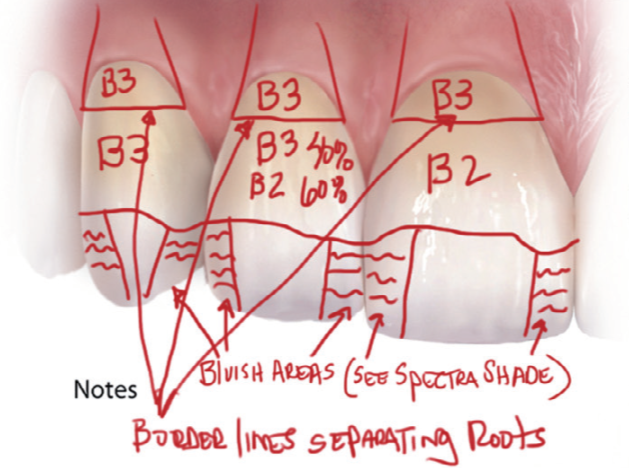
\includegraphics[width=0.5\textwidth]{grafiken/lab_card.png}
	\caption{Cutout of a lab card (Sharpling, 2015)}
	\label{fig:bild2}
\end{figure}



\begin{figure}[h]
	\centering
	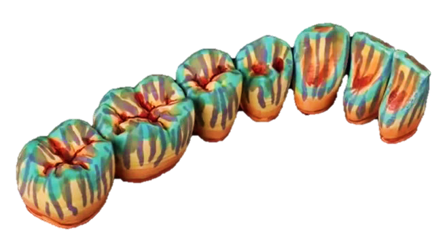
\includegraphics[width=0.6\textwidth]{grafiken/false_colored.png}
	\caption{False colored crowns after manual brushing (Zirkonzahn GmbH, 2018)}
	\label{fig:bild3}
\end{figure}


\chapter{Review of the State of the Art and Technology}
\label{sec:kritik_stand_technik}
